\documentclass[main.tex]{subfiles}

\begin{document}

\section{Result} \label{result}
In this section, we describe the training and test result for our multivarate classifier, using the gradient magnitude segmentation method in the previous section. When we manually classify the images, we output a colored border signifying the classes of the object.

%% INSERT IMAGE HERE!
\begin{figure}[!h]
  \centering
  \begin{subfigure}[b]{.4\textwidth}
    \centering
    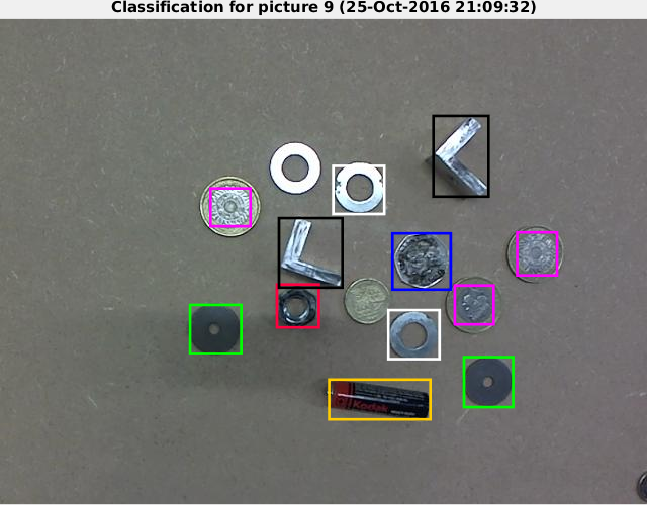
\includegraphics[width=\textwidth]{./img/srcimgs/manual_classy/ex2.png}
  \end{subfigure}
  \begin{subfigure}[b]{.4\textwidth}
    \centering
    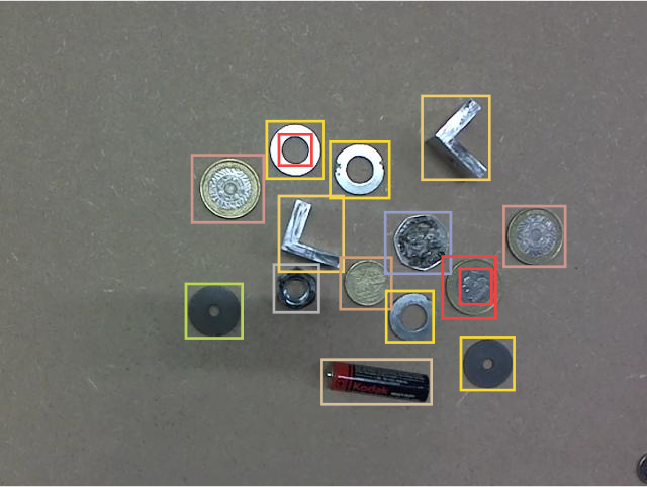
\includegraphics[width=\textwidth]{./img/srcimgs/manual_classy/ex1.png}
  \end{subfigure}
  \caption{ There difference in classification using normalised background (right) and gradient magnitude segmentation (left) is that one pound coins are almost always gone in the former, while found in the later .}
  \label{bin_image}
\end{figure}

For testing, we will be using this same format to output the data and the classification result.

\end{document}
